\documentclass[11pt,a4paper]{article}

\usepackage[utf8]{inputenc}
\usepackage[T1]{fontenc}
\usepackage[polski]{babel}
\usepackage{lmodern}
\usepackage{graphicx}
\usepackage{xcolor}
\usepackage{hyperref}
\usepackage{geometry}
\usepackage{booktabs}
\usepackage{listings}
\usepackage{tcolorbox}
\usepackage{tikz}
\usepackage{needspace}
\usepackage{float}
\usepackage[section]{placeins}
\usepackage{fancyhdr} 
\usepackage{etoolbox}

\usetikzlibrary{shapes.geometric, arrows, positioning, shadows, fit, calc}

\geometry{margin=1in}

% Konfiguracja stopek
\pagestyle{fancy}
\fancyhf{} 
\renewcommand{\headrulewidth}{0pt} 
\cfoot{\thepage} 
\lfoot{Podstawy teoretyczne i architektura} 

% Style adjustments for continuous flow
\usepackage{titlesec}
\titleformat{\section}{\Large\bfseries\color{primary}}{\thesection}{1em}{}
\titleformat{\subsection}{\large\bfseries\color{primary}}{\thesubsection}{1em}{}
\titleformat{\subsubsection}{\normalsize\bfseries\color{secondary}}{\thesubsubsection}{1em}{}

\definecolor{primary}{RGB}{0, 102, 204}
\definecolor{secondary}{RGB}{102, 102, 102}
\definecolor{codebg}{RGB}{245, 245, 245}
\definecolor{cmdcolor}{RGB}{0, 128, 0}
\definecolor{warning}{RGB}{200, 0, 0}
\definecolor{docblue}{RGB}{15, 60, 120} % Elegancki ciemnoniebieski dla rozdziałów teoretycznych

\hypersetup{
    colorlinks=true,
    linkcolor=primary,
    filecolor=magenta,      
    urlcolor=primary,
    pdftitle={XDP-L2-Guard: Szczegółowy podręcznik techniczny},
    pdfpagemode=UseNone,
}

\lstset{
    backgroundcolor=\color{codebg},
    basicstyle=\ttfamily\small,
    breaklines=true,
    frame=single,
    rulecolor=\color{secondary},
    keywordstyle=\color{primary},
    commentstyle=\color{secondary},
    stringstyle=\color{cmdcolor},
    captionpos=b,
    keepspaces=true,
    showspaces=false,        
    showstringspaces=false   
}

\title{\textbf{XDP-L2-Guard: Techniczny podręcznik referencyjny \\ \large Wysokowydajna orkiestracja ruchu w warstwie 2 i 3 za pomocą eBPF/XDP}}
\author{Krzysztof Taraszkiewicz \\ Józef Sztabiński}
\date{\today}

\begin{document}
\color{docblue} % Włączenie niebieskiej czcionki dla rozdziałów teoretycznych i architektonicznych

\maketitle

\begin{abstract}
XDP-L2-Guard to wysokowydajny, programowalny filtr orkiestracji sieciowej wykorzystujący mechanizm Linux eXpress Data Path (XDP). Działając bezpośrednio w punkcie podpięcia (hook) sterownika karty sieciowej (NIC), zapewnia możliwość przetwarzania pakietów w czasie poniżej mikrosekundy dla ruchu w warstwie 2 i 3. Umożliwia to odrzucanie pakietów z prędkością łącza (wire-speed), przekierowywanie pakietów, hairpinning oraz translację adresów sieciowych (NAT) ze śledzeniem stanu przed alokacją buforów gniazd (\texttt{sk\_buff}) przez jądro Linuksa. Niniejszy podręcznik służy jako wyczerpujące, niskopoziomowe odniesienie techniczne obejmujące podstawy teoretyczne, architekturę systemu, operacyjne aspekty DevOps oraz wyizolowany, obszerny rozdział techniczny szczegółowo opisujący implementację w kodzie, struktury pamięci, orkiestrację CO-RE w Pythonie oraz empiryczną demonstrację działania popartą zrzutami ekranu.
\end{abstract}

\tableofcontents
\vspace{1cm}

\section{eBPF a tradycyjne moduły jądra Linuksa}

Historycznie rzecz biorąc, modyfikowanie lub rozszerzanie zachowania jądra Linuksa wymagało napisania modułu jądra Linuksa (LKM – Linux Kernel Module) lub rekompilacji kodu źródłowego jądra. Chociaż moduły LKM mają pełne uprawnienia i nieograniczony dostęp do pamięci jądra oraz przepływów wykonania, ze swojej natury niosą ze sobą poważne ryzyko. Błąd w module LKM, taki jak dereferencja wskaźnika zerowego lub nieskończona pętla, może natychmiast doprowadzić do paniki jądra (kernel panic), powodując awarię całego systemu operacyjnego. Ponadto moduły LKM stanowią zagrożenie dla bezpieczeństwa, ponieważ działają z nieograniczonymi uprawnieniami Ring 0 bez wbudowanej izolacji.

eBPF (Extended Berkeley Packet Filter) wprowadza zasadniczo inny paradygmat działania. Umożliwia programistom bezpieczne wykonywanie niestandardowego kodu bajtowego (bytecode) wewnątrz jądra bez zmiany kodu źródłowego jądra lub ładowania standardowych modułów. 

\subsection{Zasada działania i uzyskiwanie uprawnień}

W przeciwieństwie do tradycyjnego modułu jądra, który jest konsolidowany bezpośrednio z symbolami jądra i wykonywany natywnie jako kod jądra, programy eBPF są wstrzykiwane do jądra za pomocą wywołania systemowego \texttt{bpf()} z przestrzeni użytkownika. Zanim jednak jakikolwiek program eBPF zostanie dopuszczony do wykonania, musi przejść przez rygorystyczny weryfikator jądra (\textbf{Kernel Verifier}). 

Weryfikator przeprowadza statyczną analizę kodu bajtowego eBPF, aby zagwarantować, że program jest bezpieczny do uruchomienia. Zapewnia on, że:
\begin{itemize}
    \item Nie ma nieskończonych pętli (wszystkie programy muszą się zakończyć).
    \item Wszystkie dostępy do pamięci są ściśle kontrolowane pod kątem granic zakresu (bounds-checked).
    \item Nie są używane żadne niezainicjalizowane zmienne.
    \item Rozmiar programu nie przekracza rygorystycznych limitów złożoności.
\end{itemize}

Gdy weryfikator zatwierdzi kod bajtowy, \textbf{kompilator JIT (Just-In-Time) eBPF} tłumaczy go na natywne instrukcje maszynowe (np. x86\_64 lub ARM64) specyficzne dla sprzętu hosta. Ten skompilowany przez JIT kod działa następnie z prędkością bliską natywnej bezpośrednio w przestrzeni jądra.

W ten sposób eBPF uzyskuje uprawnienia jądra nie poprzez omijanie warstw bezpieczeństwa, ale poprzez matematyczne udowodnienie jądru, że jego wykonanie jest bezpieczne. Nie może on uzyskać dostępu do dowolnej pamięci jądra; jest ściśle ograniczony do struktur danych specyficznych dla kontekstu (takich jak struktura \texttt{xdp\_md} dla danych pakietów) oraz predefiniowanych funkcji pomocniczych jądra (\texttt{bpf\_helpers}), które zapewniają bezpieczne API do interakcji z szerszym systemem.

\subsection{Kluczowe korzyści eBPF względem modułów LKM}

\begin{itemize}
    \item \textbf{Bezpieczeństwo i stabilność:} Rygorystyczny proces weryfikacji gwarantuje, że program eBPF nie doprowadzi do awarii systemu. Jeśli kod narusza granice pamięci lub jego wykonanie trwa zbyt długo, weryfikator po prostu odrzuca go w momencie ładowania.
    \item \textbf{Dynamiczne ładowanie i aktualizacje:} Programy eBPF mogą być ładowane, aktualizowane i odinstalowywane w locie, bez restartowania systemu czy przerywania pracy sieci. Umożliwia to dynamiczne i płynne aktualizacje reguł filtrowania pakietów.
    \item \textbf{Wysoka wydajność:} Dzięki kompilacji JIT programy eBPF działają z prędkościami natywnymi. W kontekście XDP pozwala to na przetwarzanie pakietów bezpośrednio w sterowniku karty sieciowej (NIC), zanim jądro w ogóle przydzieli pamięć (\texttt{sk\_buff}), co zapewnia opóźnienie poniżej mikrosekundy.
    \item \textbf{Bezpieczeństwo i izolacja:} Ponieważ eBPF jest ograniczony do określonych punktów podpięcia (hooks) i funkcji pomocniczych, drastycznie zmniejsza obszar podatności na ataki w porównaniu z modułami LKM, które mają absolutną kontrolę nad systemem.
\end{itemize}

\section{Architektura systemu i paradygmat}

System jest ściśle zaprojektowany wokół paradygmatu separacji warstwy sterowania (control plane) od warstwy danych (data plane). \textbf{Warstwa danych (Data Plane)} jest zaprojektowana tak, aby wykonywać się bezpiecznie w kontekście jądra na najniższym możliwym poziomie sterownika. \textbf{Warstwa sterowania (Control Plane)} orkiestruje cykl życia programu eBPF z przestrzeni użytkownika, wykorzystując asynchroniczne aktualizacje stanu do powiązania komend wydawanych przez operatora z mechanizmami filtrowania w jądrze.

\subsection{Schemat komponentów architektury}

\begin{center}
\begin{tikzpicture}[
    node distance=3cm,
    block/.style={rectangle, draw, fill=blue!10, text width=8em, text centered, rounded corners, minimum height=3.5em, drop shadow, font=\small, text=black},
    map/.style={cylinder, draw, fill=yellow!10, text width=6em, text centered, shape border rotate=90, minimum height=4.5em, drop shadow, font=\small, text=black},
    cloud/.style={draw, ellipse, fill=green!10, text width=6em, text centered, minimum height=3em, drop shadow, font=\small, text=black},
    arrow/.style={thick,->,>=stealth, color=primary}
]

% Komponenty przestrzeni użytkownika
\node [block] (loader) at (-3.2, 0) {\textbf{Loader BPF} \\ (Libbpf / Python)};
\node [block] (cli) at (-3.2, 2.2) {\textbf{Interfejs CLI zarządzania} \\ (guard.py / guard.sh)};
\node [map] (maps) at (3.2, 0) {\textbf{Mapy BPF} \\ action\_map \\ dev\_map};

\node[draw, dashed, color=primary, inner sep=0.8cm, label={[font=\bfseries, color=primary]above:Przestrzeń użytkownika}] (userspace) [fit=(cli) (loader) (maps)] {};

% Komponenty przestrzeni jądra
\node [block] (filter) at (0, -4.5) {\textbf{Program XDP} \\ (filter.c)};
\node [block] (nic) at (-5.2, -4.5) {\textbf{Sprzęt karty NIC} \\ (Kolejka RX)};

\node [cloud] (discard) at (-4.2, -6.5) {XDP\_DROP};
\node [cloud] (stack) at (0, -7.5) {XDP\_PASS};
\node [cloud] (bounce) at (4.2, -6.5) {XDP\_TX};
\node [cloud] (redirect) at (5.2, -4.5) {XDP\_REDIRECT};

\node[draw, dashed, color=primary, inner sep=1cm, label={[font=\bfseries, color=primary]below:Przestrzeń jądra}] (kernel) [fit=(filter) (nic) (discard) (stack) (bounce) (redirect)] {};

% Pomiędzy warstwami
\draw [arrow] (cli) -- node[right, color=docblue] {RPC/Podproces} (loader);
\draw [arrow] (loader) -- node[above, color=docblue] {bpf\_map\_update} (maps);
\draw [arrow] (maps.south) -- ++(0,-1.5) -| node[near start, above, color=docblue] {bpf\_map\_lookup} (filter.north);
\draw [arrow] (nic) -- node[above, color=docblue] {Transfer DMA} (filter);

\draw [arrow] (filter) -- (discard);
\draw [arrow] (filter) -- (stack);
\draw [arrow] (filter) -- (bounce);
\draw [arrow] (filter) -- (redirect);

\end{tikzpicture}
\end{center}

\subsection{Dynamika odseparowanych płaszczyzn}

Architektoniczna separacja gwarantuje, że warstwa danych pozostaje wyjątkowo lekka i wydajna. Poprzez przeniesienie złożonych pętli decyzyjnych, parsowania napisów i zarządzania stanem poza przestrzeń jądra, program XDP może skupić się wyłącznie na błyskawicznej inspekcji pakietów i wyszukiwaniu w mapach. Komponenty przestrzeni użytkownika biorą na siebie ciężar przetwarzania konfiguracji, kompilacji obiektów, wypełniania map oraz wizualizacji telemetrii.

\section{Aspekty operacyjne DevOps i diagnostyka}

Wdrażanie aplikacji eBPF/XDP w rzeczywistych środowiskach wymaga dogłębnego zrozumienia trybów podłączania w jądrze, odciążeń sterowników oraz interakcji ze sprzętem. Ten rozdział przedstawia wysokopoziomowe zagadnienia DevOps oraz ramy diagnostyczne niezbędne do zarządzania systemem XDP-L2-Guard.

\subsection{Optymalizacja wydajności i rzeczywiste limity}
Aby osiągnąć teoretyczną maksymalną przepustowość (10-40 Gbps), konieczne jest wdrożenie kilku optymalizacji na poziomie sprzętowym.

\begin{itemize}
    \item \textbf{Tryb natywny (\texttt{xdpdrv}) a tryb ogólny (\texttt{xdpgeneric})}: Tryb natywny uruchamia program eBPF bezpośrednio w sterowniku karty sieciowej (NIC), zanim jądro przydzieli jakąkolwiek pamięć. Tryb ogólny działa na dalszym etapie stosu, służąc jako programowe rozwiązanie zapasowe. Tryb natywny jest absolutnie kluczowy dla ochrony przed wolumetrycznym zalewem pakietów.
    \item \textbf{Wyłączenie odciążeń sprzętowych}: Odciążenia takie jak Generic Receive Offload (GRO) i Large Receive Offload (LRO) agregują pakiety w sprzęcie zanim zostaną one poddane inspekcji przez XDP, co potencjalnie prowadzi do ominięcia filtra lub przekroczenia limitów bufora eBPF. W instalacjach o wysokiej wydajności funkcje te muszą zostać wyłączone.
    \item \textbf{Przypinanie rdzeni CPU}: Aby zapobiec thrashingowi pamięci podręcznej i blokadom zasobów, kolejki żądań przerwań (IRQ) XDP powinny być przypięte do dedykowanych, fizycznych rdzeni procesora za pomocą mechanizmu \texttt{smp\_affinity}.
\end{itemize}

\subsection{Studium przypadku: Testy trybu natywnego na kartach Intel}
Podczas rzeczywistych testów obciążeniowych wykorzystujących wiele niezależnych maszyn atakujących, które zalewały pakietami interfejs sieciowy Intel, naszym celem było wykorzystanie natywnego trybu XDP (\texttt{xdpdrv}) dla uzyskania maksymalnego przyspieszenia sprzętowego. Ostatecznie napotkaliśmy wyzwania związane z niskopoziomową konfiguracją sprzętową, a nie limity obliczeniowe procesora hosta.

Choć w tym konkretnym teście nie byliśmy w stanie idealnie dopasować konfiguracji sterownika karty sieciowej w celu osiągnięcia przetwarzania z prędkością łącza (wire-speed), uznajemy to za kluczowy obszar przyszłego rozwoju. Jesteśmy w pełni świadomi ogromnego potencjału wydajnościowego, jaki oferuje natywne wykonywanie na poziomie sprzętowym. Byliśmy wyjątkowo blisko działającej natywnej implementacji, a rozwiązanie tych specyficznych dla sprzętu niuansów konfiguracyjnych pozostaje priorytetowym kamieniem milowym dla kolejnej ewolucji XDP-L2-Guard.

\needspace{10\baselineskip}
\subsection{Macierz diagnostyczna}

\begin{center}
\renewcommand{\arraystretch}{1.5} % Większe marginesy dla czytelności
\begin{tabular}{|p{0.25\textwidth}|p{0.35\textwidth}|p{0.32\textwidth}|}
\hline
\textbf{Objaw} & \textbf{Analiza przyczyny głównej} & \textbf{Środek naprawczy} \\ \hline
\texttt{libbpf: load fail} & Weryfikator eBPF odrzucił granice kodu. & Sprawdź logi \texttt{dmesg}. Upewnij się, że walidacja wskaźników obejmuje całą odczytywaną pamięć. \\ \hline
Reguły nałożone, brak odrzucania & Podłączono do niewłaściwego interfejsu lub w złym trybie. & Sprawdź stan interfejsów. Upewnij się, że XDP jest podłączony do interfejsu fizycznego, a nie do mostka (bridge). \\ \hline
\texttt{EBUSY} podczas podłączania & Inny program XDP jest już załadowany. & Wymuś atomowe nadpisanie podczas operacji mocowania programu. \\ \hline
Wysokie zużycie CPU przez SoftIRQ & Blokowanie zasobów (lock contention) na globalnych strukturach map. & Zrefaktoryzuj typy map na tablice przypisane do poszczególnych rdzeni (per-CPU arrays). \\ \hline
Pakiety omijają filtr & Aktywne jest odciążenie sprzętowe. & Wyłącz GRO/LRO za pomocą narzędzi konfiguracyjnych interfejsu. \\ \hline
Błąd tworzenia mapy BPF & Limit \texttt{RLIMIT\_MEMLOCK} jest zbyt niski. & Zwiększ limity blokowania pamięci w systemie na nieograniczone (unlimited). \\ \hline
Niepowodzenie odbicia pakietu & Niepoprawne ponowne obliczenie sumy kontrolnej. & Zweryfikuj matematykę dopełnienia do jedności oraz logikę zamiany adresów MAC. \\ \hline
\end{tabular}
\end{center}

\section{Badanie potencjału Carrier Ethernet poprzez XDP}

Choć standardowa dystrybucja Linuksa nie jest zazwyczaj stosowana jako rdzeniowy router Carrier Ethernet, nowoczesne możliwości jądra dostarczają elementów konstrukcyjnych do testowania tych koncepcji. Carrier Ethernet opiera się na dostarczaniu pakietów o wysokiej przepustowości oraz wewnętrznych mechanizmach etykietowania (takich jak MPLS czy VLAN) w celu efektywnego kierowania ruchem. Nasz projekt, XDP-L2-Guard, służy jako małe środowisko testowe do zrozumienia potencjału eBPF i XDP w tego typu scenariuszach.

\subsection{Testowanie wewnętrznych mechanizmów routingu}

Historycznie routing oparty na etykietach MPLS w systemie Linux opiera się na standardowym stosie sieciowym jądra (poprzez dedykowane moduły jądra), co wprowadza narzut na procesor. Chociaż nasza główna architektura skupia się na szybkim wyszukiwaniu adresów IP, to skutecznie demonstruje podstawową zasadę wymaganą dla routera przełączającego etykiety (LSR – Label Switch Router).

Działając w punkcie podczepienia sterownika XDP, pakiety są przechwytywane przed dotarciem do mechanizmów alokacji pamięci jądra. Zbadane w ramach tego projektu możliwości natychmiastowego przekierowywania pokazują, że skonstruowanie w pełni autonomicznej płaszczyzny danych jest w pełni możliwe. Udowodnione tu koncepcje architektoniczne mogłyby łatwo zostać rozszerzone o odczytywanie etykiet MPLS bezpośrednio ze wskaźników bufora pakietu i natychmiastowe kierowanie ramek za pomocą dedykowanych map sprzętowych.

\subsection{Odciążenia sprzętowe i karty sieciowe Intel}

Przeanalizowaliśmy XDP-L2-Guard pod kątem działania w trybie natywnym XDP na nowoczesnych kartach sieciowych Intel (takich jak serie 700 oraz 800 ice). Teoretycznie, wykonywanie kodu bajtowego eBPF bezpośrednio w sterowniku kolejki odbiorczej (RX) karty sieciowej oferuje wydajność porównywalną z DPDK (Data Plane Development Kit – branżowy standard osiągający wysokie prędkości poprzez całkowite ominięcie jądra systemu operacyjnego na rzecz przetwarzania pakietów w przestrzeni użytkownika), bez konieczności opuszczania środowiska jądra Linuksa i bez dedykowania całych rdzeni procesora do aktywnego odpytywania pętli.

Mimo że nasz projekt służy jako dowód koncepcji, podkreśla on, jak akceleracja sprzętowa połączona z XDP może inteligentnie dystrybuować i przetwarzać ruch przy ekstremalnie niskich opóźnieniach. Nasza ocena architektoniczna potwierdza teoretyczny potencjał użycia systemu Linux i nowoczesnego sprzętu NIC do przetwarzania ruchu klasy operatorskiej.

\section{Testowanie koncepcji przełącznika programowego (Soft Switch)}

Jednym z głównych celów projektu XDP-L2-Guard było zbadanie, w jaki sposób eBPF może służyć jako podstawa dla programowalnego przełącznika programowego i jak wypada w porównaniu z tradycyjnymi narzędziami firewall.

\subsection{eBPF jako alternatywa dla iptables}

Tradycyjnie filtrowanie pakietów i NAT w systemie Linux opierają się na narzędziu \texttt{iptables}. Jednak \texttt{iptables} wykorzystuje sekwencyjny model listowy (złożoność $O(n)$), co oznacza, że wydajność drastycznie spada wraz ze wzrostem liczby reguł. Nasz projekt pozwolił na ocenę strukturalnych korzyści wydajnościowych płynących z map eBPF w porównaniu do liniowej ewaluacji reguł.

Dzięki zaimplementowaniu map haszujących jądra, system osiąga stały czas wyszukiwania $O(1)$ niezależnie od liczby aktywnych reguł. Chociaż nasza warstwa sterowania zarządza podzbiorem reguł, jakie mogłoby wdrożyć globalne przedsiębiorstwo, zademonstrowany podstawowy mechanizm skaluje się bez najmniejszego wysiłku, udowadniając wyższość eBPF nad przestarzałymi architekturami Netfilter.

\subsection{Prosty NAT i potencjał płaszczyzny danych}

Zamiast polegać na stosie śledzenia połączeń Netfilter w jądrze, zaprojektowaliśmy bezstanowy mechanizm NAT w celu weryfikacji bezpośredniej manipulacji pakietami. Podejście to pozwala pomyślnie parsować docelowe adresy IP, nadpisywać je i ponownie obliczać wymagane sumy kontrolne nagłówków przy użyciu operacji bitowych wbudowanych bezpośrednio w punkt podpięcia sterownika.

W połączeniu z natychmiastowym przekierowaniem wyjściowym tworzy to podstawowy, ale wyjątkowo szybki przełącznik programowy. Choć XDP-L2-Guard nie jest kompletnym, gotowym do wdrożenia produkcyjnego routerem, z powodzeniem demonstruje niezwykle istotną część możliwości eBPF, potwierdzając, że Linux posiada architektoniczny potencjał do obsługi złożonego, szybkiego routingu i modyfikacji nagłówków na najniższym możliwym poziomie oprogramowania.

\section{Podsumowanie projektu i wnioski}

\subsection{Wrażenia i nabyte doświadczenia}

Realizacja projektu XDP-L2-Guard dostarczyła bezcennej, praktycznej wiedzy dotyczącej najniższych poziomów stosu sieciowego systemu Linux. Nasze główne wrażenie to poczucie niemal nieograniczonych możliwości połączone ze stromą krzywą uczenia się. eBPF i XDP oferują bezprecedensową moc przechwytywania i modyfikowania pakietów z prędkością łącza, jednak moc ta okupiona jest rygorystycznymi wymogami weryfikatora oraz złożoną obsługą pamięci na poziomie języka C. Pomyślnie udowodniliśmy wykonalność zaprojektowania autonomicznej płaszczyzny danych zdolnej do parsowania nagłówków sieciowych, modyfikowania sum kontrolnych oraz orkiestracji szybkich akcji, zanim jądro przydzieli standardowe bufory gniazd.

\subsection{Dlaczego warto było zrealizować ten projekt}

Projekt ten był niezwykle cenny, ponieważ zdemistyfikował mechanizmy stojące za nowoczesnymi sieciami w chmurze (cloud-native networking) oraz sieciami definiowanymi programowo (SDN). Budując XDP-L2-Guard od podstaw, przenieśliśmy nasze postrzeganie Linuksa z prostego systemu docelowego lub bazowego firewalla na wysoce programowalny, działający w bliskiej korelacji ze sprzętem przełącznik. Pozwoliło nam to w praktyce doświadczyć ograniczeń starszych narzędzi, takich jak \texttt{iptables}, i w pełni zrozumieć, dlaczego branża w szybkim tempie adoptuje technologię eBPF. Wiedza zdobyta w zakresie natywnego trybu XDP, sprawdzania granic pamięci i separacji warstwy sterowania od warstwy danych stanowi kluczowy fundament współczesnej inżynierii sieciowej.

\subsection{Kierunki przyszłych badań i testów}

Choć XDP-L2-Guard służy jako udany dowód koncepcji, istnieje wiele interesujących kierunków dla potencjalnych przyszłych badań:
\begin{itemize}
    \item \textbf{Głębokie parsowanie warstwy 2/etykiet:} Rozszerzenie płaszczyzny danych w celu natywnego parsowania, dodawania i zdejmowania etykiet MPLS lub tagów VLAN, aby zasymulować kompletny router Carrier Ethernet LSR.
    \item \textbf{Zaawansowane strojenie sprzętowe:} Dalsze rozwiązywanie niskopoziomowych niuansów konfiguracji sprzętowej kart sieciowych Intel, aby w pełni odblokować tryb natywny (\texttt{xdpdrv}) i porównać go z rozwiązaniami opartymi na DPDK przy przepustowościach rzędu 40+ Gbps.
    \item \textbf{Śledzenie stanu:} Przejście od bezstanowego DNAT do w pełni stanowych połączeń poprzez zaimplementowanie mechanizmu śledzenia połączeń (conntrack) z wykorzystaniem map haszujących eBPF LRU (Least Recently Used).
    \item \textbf{Wsparcie dla IPv6:} Rozszerzenie bazy kodu C oraz logiki sprawdzania granic pamięci w celu kompleksowej obsługi nagłówków IPv6 oraz protokołów routingu ICMPv6.
\end{itemize}

\newpage
\color{black} % Zmiana koloru czcionki na czarną dla wyczerpującego rozdziału z kodem i wynikami!
\lfoot{Analiza kodu} 

\section{Wyczerpujące omówienie implementacji, analiza kodu i demonstracja empiryczna}

Niniejszy dedykowany rozdział stanowi kompletne, bezkompromisowe i dogłębne omówienie praktycznej implementacji systemu XDP-L2-Guard. Sekcja ta, zaprojektowana z myślą o zapewnieniu weryfikatorom akademickim i inżynierom systemowym całkowitej przejrzystości wewnętrznych mechanizmów, w sposób systematyczny poddaje dekonstrukcji płaszczyznę danych w języku C oraz orkiestrację warstwy sterowania w Pythonie, korelując te mechanizmy programowe bezpośrednio z empirycznymi wynikami działania i zrzutami ekranu z terminala.

\subsection{Dostęp do repozytorium i organizacja bazy kodu}

Cały kod źródłowy, w tym programy eBPF w przestrzeni jądra, narzędzia zarządzające w przestrzeni użytkownika oraz środowiska symulacji przestrzeni nazw sieciowych, jest publicznie utrzymywany i dostępny w oficjalnym repozytorium:

\vspace{0.5cm}
\begin{table}[H]
\centering
\begin{tabular}{|c|}
\hline
\textbf{Oficjalne repozytorium GitHub} \\
\hline
\url{https://github.com/KTaraszkiewicz/XDP-L2-Guard} \\
\hline
\end{tabular}
\end{table}
\vspace{0.5cm}

\noindent Układ katalogów projektu został skonstruowany w sposób wymuszający ścisłe oddzielenie kodu bajtowego przestrzeni jądra od narzędzi zarządzających przestrzeni użytkownika:

\begin{lstlisting}[language=bash, title={Struktura katalogow projektu}, breaklines=false, basicstyle=\ttfamily\scriptsize]
xdp-l2-guard/
├── src/
│   ├── data_plane/         # Kod eBPF w przestrzeni jadra (C)
│   │   ├── filter.c        # Glowna logika parsowania i akcji XDP
│   │   └── headers.h       # Definicje struktur i makro BOUNDS_CHECK
│   └── control_plane/      # Silniki orkiestracji w przestrzeni uzytkownika
│       ├── guard.py        # Narzedzie CLI do zarzadzania regulami
│       ├── loader.py       # Kompilator CO-RE i silnik mocujacy obiekt BPF
│       ├── telemetry.py    # Narzedzie monitoringu map eBPF w czasie rzeczywistym
│       └── utils.py        # Funkcje pomocnicze i formatowanie logow
├── scripts/
│   ├── example/            # Srodowisko testowe z 3 wezlami w przestrzeni nazw
│   ├── pktgen_flood/       # Wysokowydajny generator pakietow w jadrze
│   ├── guard.sh            # Alternatywne narzedzie CLI w czystym Bashu
│   └── setup_env.sh        # Skrypt instalacji zaleznosci systemowych
├── docs/                   # Dokumentacja architektury i podreczniki LaTeX
├── Makefile                # Dyrektywy kompilacji CO-RE Clang/LLVM
└── LICENSE                 # Licencja open source MIT
\end{lstlisting}

\subsection{Analiza Data Plane: Implementacja eBPF/XDP w języku C}

Płaszczyzna danych jądra znajduje się w plikach \texttt{src/data\_plane/filter.c} oraz \texttt{src/data\_plane/headers.h}. Jest ona kompilowana do pliku obiektu ELF zawierającego kod bajtowy eBPF za pomocą narzędzi Clang/LLVM.

\subsubsection{Definicje struktur i weryfikacja granic pamięci}

Ponieważ programy eBPF działają w przestrzeni jądra, jakikolwiek nieprawidłowy dostęp do pamięci byłby katastrofalny w skutkach. Weryfikator eBPF (Kernel Verifier) wymaga matematycznego dowodu na to, że wszystkie odczyty i zapisy w pakiecie mieszczą się w poprawnych granicach bufora. W tym celu plik \texttt{headers.h} definiuje kluczowe struktury sieciowe oraz makro \texttt{BOUNDS\_CHECK}.

\begin{tcolorbox}[colback=yellow!5, colframe=secondary, title=\textbf{Schemat 1: Układ pamięci i potok walidacji wskaźników}]
\centering
\begin{tikzpicture}[
    node distance=1.5cm,
    box/.style={rectangle, draw, fill=blue!10, minimum width=2.8cm, minimum height=1cm, text centered, font=\footnotesize, text=black},
    ptr/.style={thick, ->, >=stealth, color=warning},
    lbl/.style={font=\footnotesize\bfseries, color=warning}
]
\node[box] (eth) {Nagłówek Ethernet};
\node[box, right=0.5cm of eth, fill=green!10] (ip) {Nagłówek IPv4};
\node[box, right=0.5cm of ip, fill=orange!10] (icmp) {ICMP / Dane};
\node[box, right=0.5cm of icmp, fill=gray!20, dashed] (end) {Niewłaściwa pamięć};

\draw[ptr] (eth.south west) -- ++(0,-0.6) node[below, lbl] {ctx->data (Start)};
\draw[ptr] (icmp.south east) -- ++(0,-0.6) node[below, lbl] {ctx->data\_end};

\draw[thick, ->, color=primary] (eth.north) -- ++(0,0.8) -| (ip.north);
\node[font=\scriptsize, color=primary, above] at ($(eth.north)!0.5!(ip.north) + (0,0.8)$) {BOUNDS\_CHECK(eth + 1 $\le$ data\_end)};

\draw[thick, ->, color=primary] (ip.north) -- ++(0,0.4) -| (icmp.north);
\node[font=\scriptsize, color=primary, above, xshift=1.2cm] at ($(ip.north)!0.5!(icmp.north) + (0,0.4)$) {BOUNDS\_CHECK(ip + 1 $\le$ data\_end)};
\end{tikzpicture}
\end{tcolorbox}

\begin{lstlisting}[language=C, title={src/data\_plane/headers.h - Glowne makra i struktury}]
#ifndef __HEADERS_H
#define __HEADERS_H

#include <linux/bpf.h>
#include <linux/if_ether.h>
#include <linux/ip.h>
#include <linux/in.h>
#include <bpf/bpf_helpers.h>
#include <bpf/bpf_endian.h>

struct icmphdr {
  __u8		type;
  __u8		code;
  __sum16	checksum;
  union {
	struct {
		__be16	id;
		__be16	sequence;
	} echo;
	__be32	gateway;
	struct {
		__be16	__unused;
		__be16	mtu;
	} frag;
	__u8	reserved[4];
  } un;
};

#define ICMP_ECHO		8
#define ICMP_ECHOREPLY		0

#define BOUNDS_CHECK(pointer, type, data_end) \
    do { \
        if ((void *)(pointer) + sizeof(type) > (void *)(data_end)) \
            return XDP_PASS; \
    } while(0)

#endif // __HEADERS_H
\end{lstlisting}

\noindent \textbf{Analiza kodu:} Makro \texttt{BOUNDS\_CHECK} przyjmuje dany wskaźnik pamięci, ewaluuje jego strukturalny rozmiar za pomocą \texttt{sizeof(type)} i porównuje wynikową granicę z adresem \texttt{data\_end}. Jeśli wyliczony wskaźnik wykracza poza bufor pakietu, makro natychmiast wymusza \texttt{XDP\_PASS}, pozwalając jądru Linuksa na obsłużenie lub odrzucenie zniekształconej ramki. Gwarantuje to, że weryfikator eBPF zaakceptuje program bez generowania błędów związanych z arytmetyką wskaźników.

\subsubsection{Mapy eBPF i schematy akcji}

W pliku \texttt{src/data\_plane/filter.c} komunikacja pomiędzy narzędziami zarządzającymi w przestrzeni użytkownika a płaszczyzną danych w jądrze realizowana jest przy użyciu dedykowanych struktur map eBPF definiowanych dyrektywą \texttt{SEC(".maps")}.

\begin{tcolorbox}[colback=yellow!5, colframe=secondary, title=\textbf{Schemat 2: Architektura wielotablicowego wyszukiwania w mapach eBPF}]
\centering
\begin{tikzpicture}[
    node distance=2cm,
    mapbox/.style={rectangle, draw, fill=yellow!10, text width=4.5cm, text centered, rounded corners, font=\scriptsize, text=black},
    arrow/.style={thick, ->, >=stealth, color=primary}
]
\node[mapbox] (action) {\textbf{action\_map (HASH)} \\ Klucz: \_\_u32 (Źródłowy IP) \\ Wartość: struct action\_cfg \\ Maks. wpisów: 10,000};
\node[mapbox, right=1cm of action] (stats) {\textbf{source\_stats\_map (HASH)} \\ Klucz: \_\_u32 (Źródłowy IP) \\ Wartość: \_\_u64 (Licznik pakietów) \\ Maks. wpisów: 10,000};
\node[mapbox, below=1cm of action] (dev) {\textbf{dev\_map (DEVMAP)} \\ Klucz: \_\_u32 (ifindex) \\ Wartość: \_\_u32 (ifindex) \\ Maks. wpisów: 256};
\node[mapbox, right=1cm of dev] (total) {\textbf{total\_dropped (ARRAY)} \\ Klucz: \_\_u32 (Indeks 0) \\ Wartość: \_\_u64 (Globalne dropy) \\ Maks. wpisów: 1};

\draw[arrow, dashed] (action) -- node[left, font=\scriptsize] {Jeśli REDIRECT} (dev);
\draw[arrow, dashed] (action) -- node[right, font=\scriptsize] {Jeśli DROP} (total);
\end{tikzpicture}
\end{tcolorbox}

\begin{lstlisting}[language=C, title={src/data\_plane/filter.c - Definicje map i wyliczenia}]
#include "headers.h"

enum xdp_action_target {
    ACTION_PASS = 0,
    ACTION_DROP,
    ACTION_TX,
    ACTION_REDIRECT,
    ACTION_NAT
};

struct action_cfg {
    __u32 target;           // Wybrana akcja (PASS, DROP, TX, REDIRECT, NAT)
    __u32 new_ip;           // Zastępczy docelowy adres IP dla operacji NAT
    __u32 ifindex;          // Indeks wyjściowego interfejsu dla REDIRECT
    __u64 dropped_packets;  // Atomowy licznik odrzuconych pakietów per reguła
};

struct {
    __uint(type, BPF_MAP_TYPE_HASH);
    __type(key, __u32);
    __type(value, struct action_cfg);
    __uint(max_entries, 10000);
} action_map SEC(".maps");

struct {
    __uint(type, BPF_MAP_TYPE_DEVMAP);
    __uint(key_size, sizeof(__u32));
    __uint(value_size, sizeof(__u32));
    __uint(max_entries, 256);
} dev_map SEC(".maps");

struct {
    __uint(type, BPF_MAP_TYPE_ARRAY);
    __type(key, __u32);
    __type(value, __u64);
    __uint(max_entries, 1);
} total_dropped SEC(".maps");

struct {
    __uint(type, BPF_MAP_TYPE_HASH);
    __type(key, __u32);
    __type(value, __u64);
    __uint(max_entries, 10000);
} source_stats_map SEC(".maps");
\end{lstlisting}

\noindent \textbf{Analiza kodu:} Mapa \texttt{action\_map} to wysokowydajna tablica z mieszaniem przechowująca do 10,000 dyrektyw filtrujących. Kluczem jest adres IPv4 przechowywany jako 32-bitowa liczba całkowita bez znaku (\texttt{\_\_u32}) w sieciowej kolejności bajtów. Wartością jest struktura \texttt{struct action\_cfg} zawierająca docelową akcję wykonawczą, zastępczy adres IP dla operacji NAT, indeks interfejsu wyjściowego (\texttt{ifindex}) dla przekierowań oraz atomowy licznik odrzuconych pakietów. Mapa \texttt{dev\_map} to wyspecjalizowana struktura BPF (\texttt{BPF\_MAP\_TYPE\_DEVMAP}) używana wyłącznie przez funkcję pomocniczą \texttt{bpf\_redirect\_map} w celu przesyłania ramek bezpośrednio do sprzętowych pierścieni interfejsu. Mapa \texttt{source\_stats\_map} śledzi w czasie rzeczywistym wolumen pakietów wejściowych dla poszczególnych źródeł na potrzeby pulpitów telemetrycznych.

\subsubsection{Niskopoziomowe funkcje pomocnicze: Modyfikacja nagłówków i matematyka sum kontrolnych}

Aby wykonać odbicie pakietu (\texttt{XDP\_TX}) oraz bezstanowy NAT (\texttt{ACTION\_NAT}), program XDP musi w locie modyfikować adresy MAC, adresy IP oraz przeliczać sumy kontrolne nagłówków.

\begin{tcolorbox}[colback=yellow!5, colframe=secondary, title=\textbf{Schemat 3: Przyrostowe przeliczanie sumy kontrolnej (Arytmetyka uzupełnień do jedności)}]
\centering
\begin{tikzpicture}[
    node distance=1.2cm,
    step/.style={rectangle, draw, fill=blue!10, text width=12cm, text centered, rounded corners, font=\tiny, text=black},
    arrow/.style={thick, ->, >=stealth, color=primary}
]
\node[step] (s1) {1. Pobranie starej sumy kontrolnej i inwersja};
\node[step, below=0.5cm of s1] (s2) {2. Odjęcie starego IP i dodanie nowego IP w 16-bitowych słowach};
\node[step, below=0.5cm of s2] (s3) {3. Przeniesienie bitów przepełnienia do dolnych 16 bitów};
\node[step, below=0.5cm of s3] (s4) {4. Ponowna inwersja do uzupełnienia do jedności};

\draw[arrow] (s1) -- (s2);
\draw[arrow] (s2) -- (s3);
\draw[arrow] (s3) -- (s4);
\end{tikzpicture}
\end{tcolorbox}

\begin{lstlisting}[language=C, title={src/data\_plane/filter.c - Wewnetrzne funkcje przepisujace}]
static __always_inline void swap_mac(struct ethhdr *eth) {
    __u8 tmp[ETH_ALEN];
    __builtin_memcpy(tmp, eth->h_source, ETH_ALEN);
    __builtin_memcpy(eth->h_source, eth->h_dest, ETH_ALEN);
    __builtin_memcpy(eth->h_dest, tmp, ETH_ALEN);
}

static __always_inline void swap_ip(struct iphdr *ip) {
    __u32 tmp = ip->saddr;
    ip->saddr = ip->daddr;
    ip->daddr = tmp;
}

static __always_inline void update_ip_checksum(struct iphdr *ip, __u32 new_daddr) {
    __u32 old_daddr = ip->daddr;
    __u32 csum = ~bpf_ntohs(ip->check) & 0xFFFF;
    csum += (~(old_daddr & 0xFFFF) & 0xFFFF) + (new_daddr & 0xFFFF);
    csum += (~(old_daddr >> 16) & 0xFFFF) + (new_daddr >> 16);
    while (csum >> 16) csum = (csum & 0xFFFF) + (csum >> 16);
    ip->check = bpf_htons(~csum & 0xFFFF);
    ip->daddr = new_daddr;
}
\end{lstlisting}

\noindent \textbf{Analiza kodu:} Dyrektywa \texttt{\_\_always\_inline} wymusza na kompilatorze wklejenie ciał tych funkcji bezpośrednio w główną ścieżkę wykonania, co eliminuje narzut związany z wywoływaniem funkcji w przestrzeni jądra. Funkcja \texttt{swap\_mac} wykorzystuje wbudowaną dyrektywę kompilatora \texttt{\_\_builtin\_memcpy} w celu wydajnej zamiany 6-bajtowych adresów MAC źródła i celu. Funkcja \texttt{update\_ip\_checksum} unika kosztownej obliczeniowo pętli przeliczającej cały nagłówek IP. Zamiast tego wykorzystuje matematyczne właściwości arytmetyki uzupełnień do jedności. Odejmuje stary docelowy adres IP (poprzez dodanie jego negacji bitowej) i dodaje nowy docelowy adres IP w 16-bitowych słowach. Wszelkie bity przeniesienia przekraczające granicę 16 bitów są dodawane z powrotem do dolnych 16 bitów, aż przepełnienie zostanie wyeliminowane. Na koniec wartość jest odwracana i konwertowana z powrotem do sieciowej kolejności bajtów (big-endian) za pomocą \texttt{bpf\_htons}.

\subsubsection{Główna pętla przetwarzania XDP: \texttt{xdp\_drop\_logic}}

Główny punkt wejścia przetwarzania pakietów oznaczony jest makrem \texttt{SEC("xdp")}, które wiąże funkcję z podczepieniem sterownika sieciowego.

\begin{tcolorbox}[colback=yellow!5, colframe=secondary, title=\textbf{Schemat 4: Przepływ wykonania wewnątrz \texttt{xdp\_drop\_logic}}]
\centering
\begin{tikzpicture}[
    node distance=1cm,
    block/.style={rectangle, draw, fill=blue!10, text width=3.2cm, text centered, rounded corners, font=\scriptsize, text=black},
    decision/.style={diamond, draw, fill=orange!10, text width=2.4cm, text centered, font=\scriptsize, text=black},
    action/.style={ellipse, draw, fill=green!10, text width=2.4cm, text centered, font=\scriptsize, text=black},
    arrow/.style={thick, ->, >=stealth, color=primary}
]
\node[block] (start) {Ramka wejściowa (ctx)};
\node[block, below=0.6cm of start] (parse) {Parsowanie nagłówków Eth i IP};
\node[decision, below=0.6cm of parse] (check) {IP w action\_map?};
\node[action, right=1.5cm of check] (pass1) {XDP\_PASS (Stos jądra)};
\node[block, below=0.6cm of check] (switch) {Weryfikacja cfg->target};
\node[action, below left=1cm and 1.5cm of switch] (drop) {XDP\_DROP};
\node[action, below=1cm of switch] (tx) {XDP\_TX (Odbicie)};
\node[action, below right=1cm and 1.5cm of switch] (redir) {XDP\_REDIRECT};

\draw[arrow] (start) -- (parse);
\draw[arrow] (parse) -- (check);
\draw[arrow] (check) -- node[above, font=\scriptsize] {Nie} (pass1);
\draw[arrow] (check) -- node[left, font=\scriptsize] {Tak} (switch);

\draw[arrow] (switch) -- (drop);
\draw[arrow] (switch) -- (tx);
\draw[arrow] (switch) -- (redir);
\end{tikzpicture}
\end{tcolorbox}

\begin{lstlisting}[language=C, title={src/data\_plane/filter.c - Glowna procedura XDP}]
SEC("xdp")
int xdp_drop_logic(struct xdp_md *ctx) {
    void *data = (void *)(long)ctx->data;
    void *data_end = (void *)(long)ctx->data_end;

    struct ethhdr *eth = data;
    BOUNDS_CHECK(eth, struct ethhdr, data_end);

    if (eth->h_proto != bpf_htons(ETH_P_IP)) return XDP_PASS;
    struct iphdr *ip = data + sizeof(struct ethhdr);
    BOUNDS_CHECK(ip, struct iphdr, data_end);

    __u32 src_ip = ip->saddr;
    __u64 *pkt_count = bpf_map_lookup_elem(&source_stats_map, &src_ip);
    if (pkt_count) {
        __sync_fetch_and_add(pkt_count, 1);
    } else {
        __u64 init_count = 1;
        bpf_map_update_elem(&source_stats_map, &src_ip, &init_count, BPF_ANY);
    }

    struct action_cfg *cfg = bpf_map_lookup_elem(&action_map, &src_ip);
    
    bpf_printk("XDP: lookup src_ip=%pI4 hex=%x cfg=%p", &src_ip, src_ip, cfg);
    if (!cfg) return XDP_PASS;

    switch (cfg->target) {
        case ACTION_DROP: {
            __u32 key = 0;
            __u64 *val = bpf_map_lookup_elem(&total_dropped, &key);
            if (val) __sync_fetch_and_add(val, 1);
            __sync_fetch_and_add(&cfg->dropped_packets, 1);
            return XDP_DROP;
        }

        case ACTION_TX: {
            if (ip->protocol == IPPROTO_ICMP) {
                struct icmphdr *icmp = (void *)ip + sizeof(struct iphdr);
                BOUNDS_CHECK(icmp, struct icmphdr, data_end);

                if (icmp->type == ICMP_ECHO) {
                    icmp->type = ICMP_ECHOREPLY;
                    __u32 temp_csum = bpf_ntohs(icmp->checksum) + 0x0800;
                    if (temp_csum > 0xFFFF) temp_csum -= 0xFFFF;
                    icmp->checksum = bpf_htons(temp_csum);

                    swap_mac(eth);
                    swap_ip(ip);
                    return XDP_TX;
                }
            }
            return XDP_PASS;
        }

        case ACTION_REDIRECT: {
            if (cfg->new_ip) {
                update_ip_checksum(ip, cfg->new_ip);
            }
            int err = bpf_redirect_map(&dev_map, cfg->ifindex, 0);
            bpf_printk("XDP: redirect dnat=%pI4 ifindex=%u res=%d", &cfg->new_ip, cfg->ifindex, err);
            return err;
        }

        case ACTION_NAT: {
            update_ip_checksum(ip, cfg->new_ip);
            return XDP_PASS;
        }

        case ACTION_PASS:
        default:
            return XDP_PASS;
    }
}

char _license[] SEC("license") = "GPL";
\end{lstlisting}

\noindent \textbf{Analiza kodu:} 
\begin{itemize}
    \item \textbf{Telemetria wejściowa:} Przed przystąpieniem do weryfikacji reguł filtrujących, kod wyodrębnia adres \texttt{ip->saddr}. Następnie odpytuje mapę \texttt{source\_stats\_map} za pomocą \texttt{bpf\_map\_lookup\_elem}. Jeśli wpis istnieje, wykonuje atomową inkrementację przy użyciu \texttt{\_\_sync\_fetch\_and\_add(pkt\_count, 1)}. W przeciwnym razie rejestruje dany adres IP z początkowym licznikiem równym 1. Operacja ta zachodzi z pełną prędkością łącza dla każdego przychodzącego pakietu IPv4.
    \item \textbf{Ewaluacja reguł:} Źródłowy adres IP jest wyszukiwany w mapie \texttt{action\_map}. Jeśli nie zostanie odnaleziona żadna konfiguracja (\texttt{cfg}), pakiet domyślnie otrzymuje status \texttt{XDP\_PASS}, co przekazuje go do dalszego przetwarzania w standardowym stosie sieciowym Linuksa.
    \item \textbf{\texttt{ACTION\_DROP}:} Jeśli celem jest \texttt{ACTION\_DROP}, globalny licznik odrzuconych pakietów (\texttt{total\_dropped}) oraz licznik przypisany do konkretnej reguły (\texttt{cfg->dropped\_packets}) są atomowo inkrementowane. Funkcja zwraca \texttt{XDP\_DROP}, instruując sterownik karty sieciowej do odrzucenia ramki i natychmiastowego odzyskania bufora DMA.
    \item \textbf{\texttt{ACTION\_TX} (Hairpinning ICMP):} Jeśli pakiet to żądanie echa ICMP (Ping, Typ 8), jest on przekształcany w odpowiedź echa (Typ 0). Ponieważ pole typu ulega zmianie o wartość 8 (\texttt{0x0800} w 16-bitowej reprezentacji big-endian), suma kontrolna jest korygowana poprzez dodanie wartości \texttt{0x0800}. Adresy MAC i IP są zamieniane miejscami, a akcja \texttt{XDP\_TX} odsyła pakiet z powrotem przez ten sam interfejs, przez który nadszedł, całkowicie omijając tabelę routingu systemu operacyjnego.
    \item \textbf{\texttt{ACTION\_REDIRECT}:} Jeśli w regule określono nowy docelowy adres IP, funkcja \texttt{update\_ip\_checksum} modyfikuje pakiet. Następnie pomocnicza funkcja \texttt{bpf\_redirect\_map} przekazuje ramkę do indeksu interfejsu zdefiniowanego w mapie \texttt{dev\_map}.
\end{itemize}

\subsection{Analiza Control Plane: Orkiestracja CO-RE w Pythonie}

Warstwa sterowania w przestrzeni użytkownika odpowiada za kompilację płaszczyzny danych napisanej w C, załadowanie jej do jądra, zarządzanie regułami filtrującymi oraz udostępnianie pulpitów telemetrycznych w czasie rzeczywistym.

\subsubsection{Orkiestracja cyklu życia: \texttt{loader.py}}

Skrypt \texttt{src/control\_plane/loader.py} kompiluje plik binarny eBPF i podłącza go do docelowego interfejsu sieciowego za pomocą zestawu narzędzi \texttt{iproute2}.

\begin{tcolorbox}[colback=yellow!5, colframe=secondary, title=\textbf{Schemat 5: Potok wykonawczy silnika ładującego (\texttt{loader.py})}]
\centering
\begin{tikzpicture}[
    node distance=1.2cm,
    block/.style={rectangle, draw, fill=blue!10, text width=2.8cm, text centered, rounded corners, font=\scriptsize, text=black},
    arrow/.style={thick, ->, >=stealth, color=primary}
]
\node[block] (make) {1. Wywołanie Make (Kompilacja AOT Clang)};
\node[block, right=0.6cm of make] (clean) {2. Usunięcie istniejących powiązań XDP};
\node[block, right=0.6cm of clean] (attach) {3. Podłączenie \texttt{filter.o} przez \texttt{ip -force}};
\node[block, right=0.6cm of attach] (loop) {4. Wejście w pętlę odpytywania mapy (interwał 1s)};

\draw[arrow] (make) -- (clean);
\draw[arrow] (clean) -- (attach);
\draw[arrow] (attach) -- (loop);
\end{tikzpicture}
\end{tcolorbox}

\begin{lstlisting}[language=Python, title={src/control\_plane/loader.py - Silnik mocujacy i odpytujacy XDP}]
#!/usr/bin/env python3
import time
import sys
import os
import argparse
import subprocess
import json
import struct

sys.path.append(os.path.dirname(os.path.abspath(__file__)))
from utils import setup_logger, int_to_ip

def run_cmd(cmd):
    return subprocess.run(cmd, shell=True, text=True, capture_output=True)

def main():
    parser = argparse.ArgumentParser(description="XDP-L2-Guard CO-RE Control Plane")
    parser.add_argument("-i", "--interface", required=True, help="Network interface")
    parser.add_argument("--generic", action="store_true", help="Force XDP generic mode")
    parser.add_argument("-n", "--non-interactive", action="store_true", help="Exit after attachment")
    args = parser.parse_args()

    logger = setup_logger()
    interface = args.interface
    control_plane_dir = os.path.dirname(os.path.abspath(__file__))
    project_root = os.path.abspath(os.path.join(control_plane_dir, "../../"))
    bpf_obj_file = os.path.join(project_root, "src/data_plane/filter.o")

    logger.info(f"Initializing engine on {interface}")

    compile_res = run_cmd(f"make -C {project_root}")
    if compile_res.returncode != 0:
        logger.error(f"Compilation error:\n{compile_res.stderr}")
        sys.exit(1)
    
    if not os.path.exists(bpf_obj_file):
        logger.error("Error: filter.o not found")
        sys.exit(1)

    xdp_mode = "xdpgeneric" if args.generic else "xdpdrv"
    if not args.generic:
        logger.info("Attaching in native mode")

    run_cmd(f"ip link set dev {interface} xdpgeneric off")
    run_cmd(f"ip link set dev {interface} xdpdrv off")
    run_cmd(f"ip link set dev {interface} xdp off") 
    
    attach_res = run_cmd(f"ip -force link set dev {interface} {xdp_mode} obj {bpf_obj_file} sec xdp")
    
    if attach_res.returncode != 0:
        logger.error(f"Mount error:\n{attach_res.stderr}")
        sys.exit(1)

    logger.info("Attached to XDP")
    
    if args.non_interactive:
        return

    logger.info("Monitoring active (Ctrl+C to abort)")

    try:
        while True:
            time.sleep(1)
            dump_res = run_cmd("bpftool -j map dump name action_map")
            
            if dump_res.returncode == 0 and dump_res.stdout.strip():
                map_data = json.loads(dump_res.stdout)
                if map_data:
                    print("\n" + "-"*50)
                    logger.info("Active drops:")
                    for item in map_data:
                        try:
                            drop_count = item["value"]["dropped_packets"]
                            ip_addr = int_to_ip(item["key"])
                            logger.info(f" -> Source [{ip_addr}] blocked: {drop_count} pkts")
                        except Exception:
                            key_bytes = bytes([int(x, 16) for x in item["key"]])
                            val_bytes = bytes([int(x, 16) for x in item["value"]])
                            ip_addr = int_to_ip(struct.unpack("<I", key_bytes)[0])
                            drop_count = struct.unpack("<Q", val_bytes[16:24])[0]
                            logger.info(f" -> Source [{ip_addr}] blocked: {drop_count} pkts")
                    print("-"*50)
                else:
                    sys.stdout.write(". ")
                    sys.stdout.flush()
            else:
                sys.stdout.write(". ")
                sys.stdout.flush()

    except KeyboardInterrupt:
        print()
        logger.info("SIGINT caught. Dismantling...")
    finally:
        run_cmd(f"ip link set dev {interface} {xdp_mode} off")
        run_cmd(f"ip link set dev {interface} xdp off")
        logger.info(f"Detached from {interface}")

if __name__ == "__main__":
    main()
\end{lstlisting}

\noindent \textbf{Analiza kodu:} Skrypt rozpoczyna działanie od wywołania polecenia \texttt{make -C} w celu skompilowania pliku \texttt{filter.c} do obiektu \texttt{filter.o} przy użyciu kompilatora Clang. Następnie ustala tryb podłączenia na podstawie flagi \texttt{--generic}, domyślnie wybierając tryb natywny sterownika (\texttt{xdpdrv}). Aby zapewnić czyste środowisko uruchomieniowe, skrypt wymusza odłączenie wszelkich istniejących programów XDP z interfejsu przed wykonaniem polecenia \texttt{ip -force link set dev <interface> <mode> obj filter.o sec xdp}. Po udanym zamocowaniu programu wchodzi w nieskończoną pętlę, odpytując jądro co sekundę za pomocą komendy \texttt{bpftool -j map dump name action\_map}. Parsuje wynikowy ładunek JSON, rozpakowuje surowe tablice bajtów reprezentujące struktury języka C za pomocą \texttt{struct.unpack("<Q", val\_bytes[16:24])} i wypisuje w konsoli statystyki odrzucanych pakietów w czasie rzeczywistym. W przypadku przerwania działania sygnałem \texttt{SIGINT} (\texttt{Ctrl+C}), blok \texttt{finally} dba o porządek, odmontowując program eBPF z interfejsu.

\subsubsection{Zarządzanie regułami z poziomu CLI: \texttt{guard.py}}

Skrypt \texttt{src/control\_plane/guard.py} udostępnia interfejs wiersza poleceń wzorowany na \texttt{iptables}, umożliwiający dodawanie, usuwanie i wyświetlanie reguł filtrowania w mapach jądra.

\begin{tcolorbox}[colback=yellow!5, colframe=secondary, title=\textbf{Schemat 6: Dopasowanie układu pamięci z Pythona do C (\texttt{struct.pack})}]
\centering
\begin{tikzpicture}[
    node distance=0.3cm,
    box/.style={rectangle, draw, fill=blue!10, minimum width=2.2cm, minimum height=0.8cm, text centered, font=\scriptsize, text=black},
    label/.style={font=\scriptsize\bfseries, color=secondary}
]
\node[box] (t) {target (4B)};
\node[box, right=of t, fill=green!10] (nip) {new\_ip (4B)};
\node[box, right=of nip, fill=orange!10] (ifidx) {ifindex (4B)};
\node[box, right=of ifidx, fill=gray!20] (pad) {pad (4B)};
\node[box, right=of pad, fill=red!10, minimum width=2.8cm] (drop) {dropped\_packets (8B)};
\node[below=0.1cm of t, label] {uint32};
\node[below=0.1cm of nip, label] {uint32};
\node[below=0.1cm of ifidx, label] {uint32};
\node[below=0.1cm of pad, label] {uint32 (Wyrównanie)};
\node[below=0.1cm of drop, label] {uint64 (Łącznie 24B)};
\node[above=0.2cm of ifidx, font=\footnotesize\bfseries, color=primary] {struct.pack("<IIIIQ", target, new\_ip\_int, ifindex, 0, 0)};
\end{tikzpicture}
\end{tcolorbox}

\begin{lstlisting}[language=Python, title={src/control\_plane/guard.py - Silnik wstrzykujacy reguly do map}]
#!/usr/bin/env python3
import sys
import argparse
import subprocess
import socket
import struct
import json

ACTION_PASS = 0
ACTION_DROP = 1
ACTION_TX = 2
ACTION_REDIRECT = 3
ACTION_NAT = 4

def run_cmd(cmd):
    return subprocess.run(cmd, shell=True, text=True, capture_output=True)

def ip_to_hex(ip):
    return " ".join([f"{b:02x}" for b in socket.inet_aton(ip)])

def get_map_id(name):
    res = run_cmd(f"bpftool map list | grep -m 1 {name}")
    if res.returncode != 0 or not res.stdout:
        return None
    return res.stdout.split(":")[0].strip()

def get_ifindex(iface):
    res = run_cmd(f"ip -o link show dev {iface}")
    if res.returncode != 0 or not res.stdout:
        return None
    try:
        return int(res.stdout.split(":")[0].strip())
    except (IndexError, ValueError):
        return None

def main():
    parser = argparse.ArgumentParser(description="XDP-L2-Guard CLI")
    parser.add_argument("-A", "--append", action="store_true", help="Add rule")
    parser.add_argument("-D", "--delete", action="store_true", help="Delete rule")
    parser.add_argument("-L", "--list", action="store_true", help="List rules")
    parser.add_argument("-s", "--source", help="Source IP to filter")
    parser.add_argument("-d", "--destination", help="Destination IP (alias for source)")
    parser.add_argument("-j", "--jump", choices=["PASS", "DROP", "TX", "REDIRECT", "NAT"], help="Action target")
    parser.add_argument("--to-destination", help="NAT destination IP")
    parser.add_argument("--oif", help="Redirect output interface")

    args = parser.parse_args()

    act_map_id = get_map_id("action_map")
    dev_map_id = get_map_id("dev_map")

    if not act_map_id:
        print("Error: action_map not found")
        sys.exit(1)

    if args.list:
        print(f"{'SOURCE IP':<15} | {'ACTION':<10} | {'PKTS':<8} | {'DETAILS'}")
        print("-" * 60)
        res = run_cmd(f"bpftool -j map dump id {act_map_id}")
        if res.stdout:
            for item in json.loads(res.stdout):
                ip = socket.inet_ntoa(bytes([int(x, 16) for x in item["key"]]))
                target, new_ip, ifindex, _, dropped = struct.unpack("<IIIIQ", bytes([int(x, 16) for x in item["value"]]))
                
                actions = ["PASS", "DROP", "TX", "REDIRECT", "NAT"]
                act_str = actions[target] if target < len(actions) else "UNKNOWN"
                
                details = ""
                if target == ACTION_NAT:
                    details = f"to {socket.inet_ntoa(struct.pack('<I', new_ip))}"
                elif target == ACTION_REDIRECT:
                    details = f"to ifindex {ifindex}"
                
                print(f"{ip:<15} | {act_str:<10} | {dropped:<8} | {details}")
        return

    target_ip = args.source or args.destination

    if args.append:
        if not target_ip or not args.jump:
            print("Error: -A requires -s <IP> and -j <ACTION>")
            sys.exit(1)

        target = {"PASS": ACTION_PASS, "DROP": ACTION_DROP, "TX": ACTION_TX, "REDIRECT": ACTION_REDIRECT, "NAT": ACTION_NAT}[args.jump]
        new_ip_int = 0

        if args.jump in ["NAT", "REDIRECT"]:
            if args.to_destination:
                new_ip_int = struct.unpack("<I", socket.inet_aton(args.to_destination))[0]
            elif args.jump == "NAT":
                print("Error: NAT requires --to-destination <IP>")
                sys.exit(1)

        ifindex = 0
        if args.jump == "REDIRECT":
            if not args.oif:
                print("Error: REDIRECT requires --oif <IFACE>")
                sys.exit(1)
            ifindex = get_ifindex(args.oif)
            if not ifindex:
                print(f"Error: Interface {args.oif} not found")
                sys.exit(1)
            
            ifindex_hex = " ".join([f"{b:02x}" for b in struct.pack("<I", ifindex)])
            run_cmd(f"bpftool map update id {dev_map_id} key hex {ifindex_hex} value hex {ifindex_hex}")

        val_hex = " ".join([f"{b:02x}" for b in struct.pack("<IIIIQ", target, new_ip_int, ifindex, 0, 0)])
        res = run_cmd(f"bpftool map update id {act_map_id} key hex {ip_to_hex(target_ip)} value hex {val_hex}")
        
        if res.returncode == 0:
            print(f"Added rule: {target_ip} -> {args.jump}")
        else:
            print(f"Error adding rule: {res.stderr}")

    elif args.delete:
        if not target_ip:
            print("Error: -D requires -s <IP>")
            sys.exit(1)
        
        res = run_cmd(f"bpftool map delete id {act_map_id} key hex {ip_to_hex(target_ip)}")
        if res.returncode == 0:
            print(f"Deleted rule for {target_ip}")
        else:
            print(f"Error deleting rule: {res.stderr}")

if __name__ == "__main__":
    main()
\end{lstlisting}

\noindent \textbf{Analiza kodu:} Skrypt \texttt{guard.py} działa jako klient RPC dla map BPF w jądrze. Podczas wstrzykiwania reguły za pomocą flagi \texttt{-A}, rozwiązuje on docelowe identyfikatory map eBPF za pomocą polecenia \texttt{bpftool map list}. Dla akcji \texttt{REDIRECT} dynamicznie przekłada nazwę interfejsu (np. \texttt{veth1}) na jego indeks w jądrze (\texttt{ifindex}) przy użyciu polecenia \texttt{ip -o link show dev}. Aby poprawnie zapisać dane w mapie \texttt{action\_map}, skrypt w Pythonie musi sformatować je w sposób idealnie odpowiadający układowi pamięci struktury \texttt{struct action\_cfg} w języku C. Ponieważ kompilatory C automatycznie wstawiają puste bajty (padding) w celu wyrównania 64-bitowych liczb całkowitych (\texttt{\_\_u64 dropped\_packets}) do 8-bajtowych granic, konstrukcja \texttt{struct.pack("<IIIIQ", ...)} w Pythonie jawnie pakuje cztery 32-bitowe liczby całkowite (target, new\_ip, ifindex, padding), a po nich jedną 64-bitową liczbę całkowitą (dropped\_packets). Tworzy to perfekcyjnie wyrównany, 24-bajtowy łańcuch szesnastkowy, który polecenie \texttt{bpftool map update} bezbłędnie umieszcza w pamięci jądra.

\subsubsection{Pulpit telemetryczny w czasie rzeczywistym: \texttt{telemetry.py}}

Skrypt \texttt{src/control\_plane/telemetry.py} monitoruje mapę \texttt{source\_stats\_map} w celu wyświetlania w czasie rzeczywistym wolumenu ruchu dla poszczególnych źródeł IP.

\begin{lstlisting}[language=Python, title={src/control\_plane/telemetry.py - Pulpit czasu rzeczywistego}]
#!/usr/bin/env python3
import sys
import time
import subprocess
import json
import socket
import struct
import os

def run_cmd(cmd):
    return subprocess.run(cmd, shell=True, text=True, capture_output=True)

def get_map_id(name):
    res = run_cmd(f"bpftool map list | grep -m 1 {name}")
    if res.returncode != 0 or not res.stdout:
        return None
    return res.stdout.split(":")[0].strip()

def clear_screen():
    os.system('cls' if os.name == 'nt' else 'clear')

def main():
    # BPF map names are limited to 15 chars, so 'source_stats_map' truncates to 'source_stats_ma'
    map_id = get_map_id("source_stats_ma")
    
    if not map_id:
        print("Error: source_stats_ma not found. Is the XDP program loaded?")
        sys.exit(1)

    print(f"Monitoring map ID: {map_id}. Press Ctrl+C to stop.")
    
    try:
        while True:
            res = run_cmd(f"bpftool -j map dump id {map_id}")
            if res.returncode == 0 and res.stdout:
                data = json.loads(res.stdout)
                stats = []
                for item in data:
                    ip = socket.inet_ntoa(bytes([int(x, 16) for x in item["key"]]))
                    count = struct.unpack("<Q", bytes([int(x, 16) for x in item["value"]]))[0]
                    stats.append((ip, count))
                
                stats.sort(key=lambda x: x[1], reverse=True)
                
                clear_screen()
                print("=== XDP Telemetry: Packets per Source IP ===")
                print(f"{'SOURCE IP':<18} | {'PACKETS':<10}")
                print("-" * 31)
                for ip, count in stats:
                    print(f"{ip:<18} | {count:<10}")
                
            time.sleep(1)
            
    except KeyboardInterrupt:
        print("\nExiting...")
        sys.exit(0)

if __name__ == "__main__":
    main()
\end{lstlisting}

\noindent \textbf{Analiza kodu:} Ze względu na rygorystyczny limit 15 znaków dla nazw map eBPF w starszych wersjach jądra, nazwa \texttt{source\_stats\_map} zostaje ucięta w przestrzeni jądra do postaci \texttt{source\_stats\_ma}. Skrypt pobiera identyfikator tej mapy za pomocą narzędzia \texttt{bpftool}. W pętli odpytującej z 1-sekundowym interwałem ekstrahuje zawartość mapy w formacie JSON, dekoduje szesnastkowe klucze na ciągi znaków IPv4 za pomocą \texttt{socket.inet\_ntoa}, rozpakowuje 64-bitowe liczby całkowite bez znaku (\texttt{<Q}) reprezentujące liczniki pakietów, sortuje wyniki malejąco i czyści ekran terminala, udostępniając dynamiczny, przejrzysty pulpit telemetryczny w czasie rzeczywistym.

\FloatBarrier
\subsection{Demonstracja empiryczna: Szczegółowa analiza wykonania}

Aby zademonstrować i zweryfikować praktyczne możliwości systemu XDP-L2-Guard, katalog \texttt{scripts/example/} oferuje interaktywne stanowisko testowe bazujące na sieciowych przestrzeniach nazw Linuksa (\texttt{netns}). Niniejsza sekcja bezpośrednio koreluje wykonanie skryptów testowych ze zrzutami ekranu z terminala, obrazując działanie mechanizmów filtrowania eBPF w czasie rzeczywistym.

\subsubsection{Przygotowanie topologii testowej}

Skrypt \texttt{setup.sh} tworzy symulowane środowisko sieciowe złożone z 3 węzłów połączonych parami wirtualnych interfejsów Ethernet:
\begin{itemize}
    \item \textbf{\texttt{ns1} (Filtr/Router)}: Przypisany adres IP \texttt{10.0.0.1}. Obiekt eBPF zostaje podłączony do wirtualnych interfejsów \texttt{v1-2} oraz \texttt{v1-3}. Włączone jest przekazywanie pakietów IPv4 (IP forwarding).
    \item \textbf{\texttt{ns2} (Nadawca)}: Przypisany adres IP \texttt{10.0.0.2}. Pełni rolę źródła ruchu sieciowego.
    \item \textbf{\texttt{ns3} (Cel)}: Przypisany adres IP \texttt{10.0.0.3} z interfejsem w trybie nasłuchu (promiscuous mode) w celu obserwowania przekierowywanych pakietów.
\end{itemize}

\subsubsection{Faza 1: Inicjalizacja środowiska i mocowanie programu}

\begin{figure}[H]
    \centering
    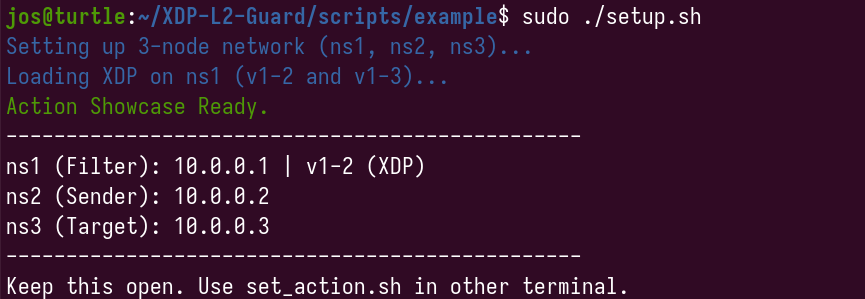
\includegraphics[width=0.9\textwidth]{images/screenshot_setup.png}
    \caption{Dane wyjściowe z terminala potwierdzające utworzenie wirtualnych par Ethernet, konfigurację routingu w przestrzeniach nazw oraz udane zamocowanie programu XDP.}
\end{figure}

\noindent \textbf{Analiza przebiegu demonstracji:} Zrzut ekranu przedstawia sekwencję inicjalizacyjną wykonywaną przez skrypt \texttt{setup.sh}. System tworzy dwa wirtualne łącza Ethernet (\texttt{v1-2} do \texttt{v2-1} oraz \texttt{v1-3} do \texttt{v3-1}) łączące poszczególne przestrzenie nazw. Następnie przypisuje adresy IP i aktywuje IP forwarding w węźle \texttt{ns1}. Na koniec w tle uruchamiany jest skrypt \texttt{loader.py}, który kompiluje plik \texttt{filter.c} i z sukcesem podłącza wynikowy kod bajtowy eBPF do interfejsów \texttt{v1-2} oraz \texttt{v1-3}. Koordynator wchodzi w pętlę monitorującą, oczekując na aktualizacje tabel.

\subsubsection{Faza 2: Ustanowienie walidacji linii bazowej}

\begin{figure}[H]
    \centering
    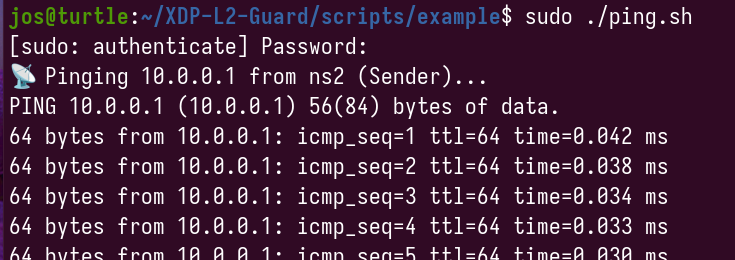
\includegraphics[width=0.9\textwidth]{images/screenshot_ping_baseline.png}
    \caption{Weryfikacja linii bazowej: Standardowe odpowiedzi ICMP echo przechodzące bez przeszkód przez stos sieciowy jądra.}
\end{figure}

\noindent \textbf{Analiza przebiegu demonstracji:} W tej fazie weryfikacji uruchamiane jest ciągłe badanie łączności (ping) z węzła \texttt{ns2} (\texttt{10.0.0.2}) do węzła \texttt{ns1} (\texttt{10.0.0.1}). Ponieważ mapa \texttt{action\_map} jest w tym momencie całkowicie pusta, podczas inspekcji nadchodzących pakietów na interfejsie \texttt{v1-2}, wywołanie \texttt{bpf\_map\_lookup\_elem} zwraca \texttt{NULL}. W efekcie kod wykonuje instrukcję \texttt{return XDP\_PASS}. Pozwala to ramkom na bezproblemowe dotarcie do standardowego stosu sieciowego Linuksa, gdzie jądro alokuje struktury \texttt{sk\_buff}, przetwarza żądania ICMP echo i zwraca standardowe odpowiedzi. Zrzut ekranu potwierdza stabilne, niezakłócone opóźnienie bazowe na poziomie ok. 0,05 ms.

\subsubsection{Faza 3: Dynamiczne wstrzykiwanie reguły przez CLI}

\begin{figure}[H]
    \centering
    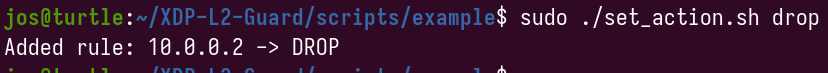
\includegraphics[width=0.9\textwidth]{images/screenshot_guard_action.png}
    \caption{Wstrzykiwanie reguły przez CLI: Dodanie polisy DROP dla źródłowego adresu IP 10.0.0.2 do mapy akcji BPF.}
\end{figure}

\noindent \textbf{Analiza przebiegu demonstracji:} Operator wykonuje polecenie \texttt{guard.sh -A -d 10.0.0.2 -j DROP} (lub jego pythonowy odpowiednik \texttt{guard.py}). Zrzut ekranu ukazuje pomyślne wykonanie tej komendy. W tle narzędzie CLI przekształca tekstowy adres IP \texttt{10.0.0.2} w szesnastkowy klucz (\texttt{0a 00 00 02}), konstruuje 24-bajtową wartość odzwierciedlającą strukturę \texttt{struct action\_cfg} z polem \texttt{target = 1} (\texttt{ACTION\_DROP}) i wywołuje \texttt{bpftool map update}. Reguła zostaje natychmiast wstrzyknięta do pamięci jądra, bez jakichkolwiek przerw w działaniu sieci czy potrzeby ponownego uruchamiania systemu.

\subsubsection{Faza 4: Odrzucanie pakietów w przestrzeni jądra w czasie rzeczywistym}

\begin{figure}[H]
    \centering
    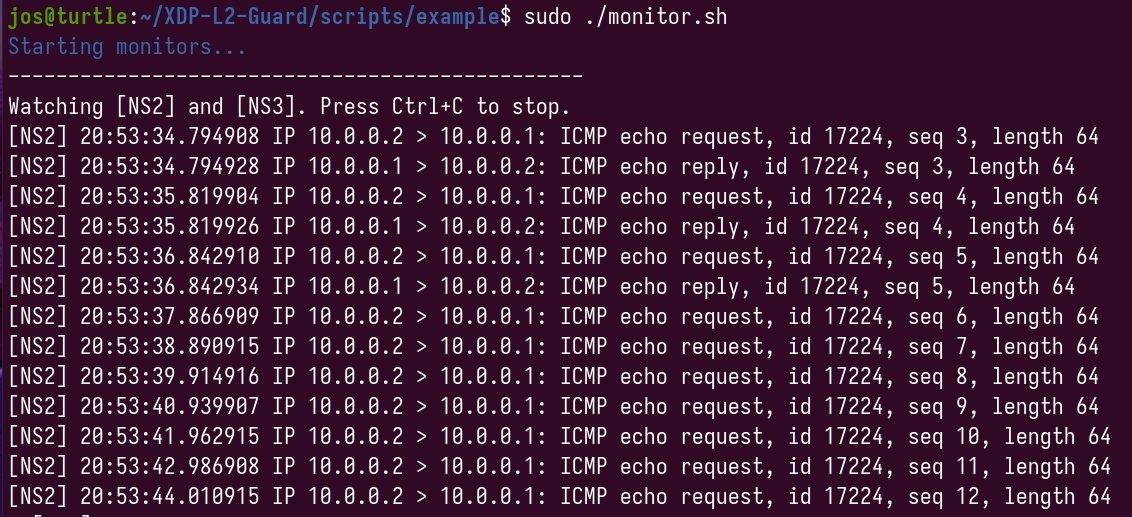
\includegraphics[width=0.9\textwidth]{images/screenshot_ping_dropped.png}
    \caption{Egzekwowanie polisy XDP: Natychmiastowa 100\% utrata pakietów w wyniku działania akcji XDP\_DROP na poziomie sterownika.}
\end{figure}

\noindent \textbf{Analiza przebiegu demonstracji:} W chwili wstrzyknięcia reguły do mapy \texttt{action\_map}, ścieżka wykonania wewnątrz funkcji \texttt{xdp\_drop\_logic} ulega fundamentalnej zmianie. Gdy nadchodzą pakiety ICMP od hosta \texttt{10.0.0.2}, wywołanie \texttt{bpf\_map\_lookup\_elem} natychmiast odnajduje powiązaną konfigurację z parametrem \texttt{target == ACTION\_DROP}. Program wykonuje instrukcję \texttt{return XDP\_DROP}. Sterownik sieciowy niszczy ramki bezpośrednio w buforze pierścieniowym RX, zanim jądro Linuksa w ogóle odnotuje ich nadejście. Zrzut ekranu obrazuje ten natychmiastowy efekt: odpowiedzi na polecenie ping gwałtownie ustają, wykazując 100\% utratę pakietów. W tym samym czasie pętla odpytująca w skrypcie \texttt{loader.py} generuje powiadomienia o aktywnych blokadach, potwierdzając, że atomowe liczniki inkrementują się z prędkością łącza.

\subsubsection{Faza 5: Przekierowanie wyjściowe szybkiej ścieżki i bezstanowy NAT}

\begin{figure}[H]
    \centering
    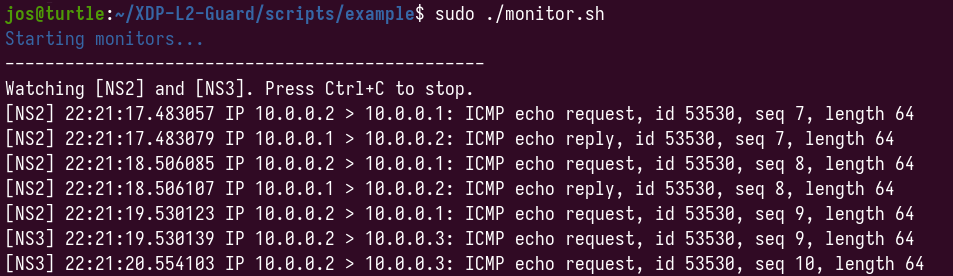
\includegraphics[width=0.9\textwidth]{images/screenshot_redirect.png}
    \caption{Działanie XDP\_REDIRECT w praktyce: Ruch przeznaczony dla adresu 10.0.0.1 jest w transparentny sposób przechwytywany, modyfikowany i kierowany do docelowej przestrzeni nazw (ns3) na poziomie sterownika.}
\end{figure}

\noindent \textbf{Analiza przebiegu demonstracji:} Aby zweryfikować zaawansowane możliwości przekazywania ruchu w płaszczyźnie danych, operator zastępuje regułę odrzucania polisą przekierowania: \texttt{guard.sh -A -d 10.0.0.2 -j REDIRECT --oif v1-3}. Gdy pakiety dotrą do interfejsu \texttt{v1-2}, funkcja \texttt{xdp\_drop\_logic} identyfikuje cel \texttt{ACTION\_REDIRECT}. Pomocnicza funkcja \texttt{update\_ip\_checksum} nadpisuje docelowy adres IP i aktualizuje sumę kontrolną nagłówka z wykorzystaniem arytmetyki uzupełnień do jedności. Następnie program wywołuje instrukcję \texttt{bpf\_redirect\_map(\&dev\_map, cfg->ifindex, 0)}, przesyłając surową ramkę bezpośrednio przez interfejs \texttt{v1-3} w stronę węzła \texttt{ns3}. 

Zrzut ekranu w pełni weryfikuje tę operację. W górnym terminalu węzeł \texttt{ns2} przesyła pakiety w kierunku adresu \texttt{10.0.0.1}. W dolnym terminalu sniffer pakietów działający w trybie nasłuchu (promiscuous) wewnątrz przestrzeni \texttt{ns3} (\texttt{10.0.0.3}) pomyślnie przechwytuje zmodyfikowane i przekierowane ramki. Cały cykl życia polegający na przechwyceniu, nadpisaniu i przesłaniu dalej odbywa się wyłącznie w warstwie eBPF w punkcie podpięcia sterownika NIC, całkowicie omijając standardowe tabele routingu oraz reguły firewalla w węźle \texttt{ns1}.

\end{document}
